%!TEX root = ../../../adrien_gomar_phd.tex

This section provides theoretical results on the
convergence of Fourier-based time methods as well
as an example motivating the use of such an approach
for the current work.

\subsection{Theoretical results}
\label{sub:spectral_accuracy}

The convergence of the spectral operator depends on
the regularity of the approximated function. Consider a function
$u(t)$ that is continuous, periodic and bounded in $[0,T]$
and let $P_N \left(u(t)\right)$ denote its truncated Fourier series
\begin{equation}
    P_N \left(u(t)\right) = \sum_{k=-N}^{N} \widehat{u}_k e^{i k\omega t}.
\end{equation}
The $\mathcal{L}_2$-norm of the error writes
\begin{equation}
   \| u \|_2 = \left(\int_0^T |u(t) - P_N \left(u(t)\right)|^2 \diff t \right)^{1/2}.
\end{equation}
If $u(t)$ is m-times continuously differentiable in $[0,T]$ ($m \geq 1$) 
and its $j$-th derivative is periodic on $[0,T]$ for all $j \leq m - 2$
then, it exists  $k_0 \in [1, N]$ such that
\begin{equation}
    \widehat{u}_k = \mathcal{O} (k^{-m}),~\textrm{for } k > k_0,
\end{equation}
where $\widehat{u}_k$ is the k-th Fourier coefficient of $u(t)$.
This equation means that, the more regular the function is,
the faster the convergence rate of the Fourier
coefficients.
The property of the error to decay exponentially as soon as 
the function is approximated by a number of harmonics greater than $k_0$, 
is called spectral accuracy~\cite{Canuto2006}. Note that
$k_0$ is not known but is rather essential for the analysis.
For $k$ below $k_0$, approximating the function $u(t)$ with its Fourier
series yields unacceptably high errors.

\subsection{Motivating example: numerical derivation of a smooth function}
\label{sec:hb_operator}

To assess the capability of the HB operator, used in the present work, to
provide accurate approximations of the time-derivative, 
we consider the simple example of a pure
five-harmonic signal of the form
\begin{equation}
    \label{eq:sum_sin}
    u(t) = \cos(\omega t) + \sin(2 \omega t) +
    \cos(3 \omega t) + \sin(4 \omega t) + \cos(5 \omega t),
\end{equation}
where $\omega = 2 \pi f$ and $f$ is the temporal frequency of
the considered phenomenon.
The analytical derivative is then
\begin{equation}
    \label{eq:sum_sin_deriv}
    \frac{\diff u}{\diff t} = 
    \omega\left[ -\sin(\omega t) + 
    2\cos(2 \omega t) -
    3\sin(3 \omega t) + 
    4\cos(4 \omega t) -
    5\sin(5 \omega t)\right].
\end{equation}
The exact derivative is compared to the approximated one obtained by applying 
the HB operator defined in Eq.~\eqref{eq:sm_hb_mono_source_term_matrix}.
Two Finite-Difference (FD) schemes are used for comparison:
a second-order centered scheme
\begin{equation}
    \frac{\diff u}{\diff t} (t=t_q) =
    \frac{u_{q+1} - u_{q-1}}{2 \Delta t} + \mathcal{O} (\Delta x^2),
    \label{eq:hb_op_center2}
\end{equation}
where $u_q = u(t_q)$ and $u_{q + 1} = u(t_{q + 1})$ and so on,
and a fourth-order centered scheme
\begin{equation}
    \frac{\diff u}{\diff t} (t=t_q) =
    \frac{-u_{q+2} + 8 u_{q+1} - 8 u_{q-1} + u_{q-2}}{12\Delta t}
    + \mathcal{O} (\Delta x^4),
    \label{eq:hb_op_center4}
\end{equation}
are also used for comparison.
For finite-difference schemes, 
we assume that the time line is discretized 
by a regular mesh of step $\Delta t$, such that $t_q = q \Delta t$.

Figure~\ref{fig:hb_operator_sample} shows the resulting approximations 
of the derivative over one period.
\begin{figure}[htp]
  \centering
  \subfigure[HB]{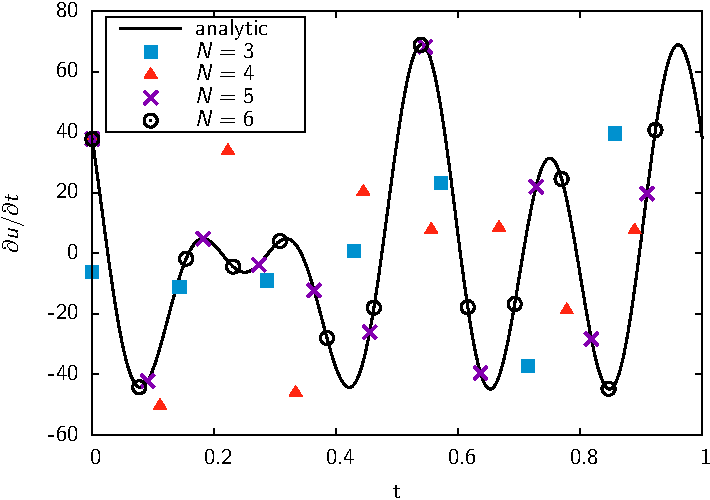
\includegraphics[width=.4\textwidth]{HB_OPERATOR_PPT_HB.pdf}}
  \subfigure[FD 2\textsuperscript{nd} order]{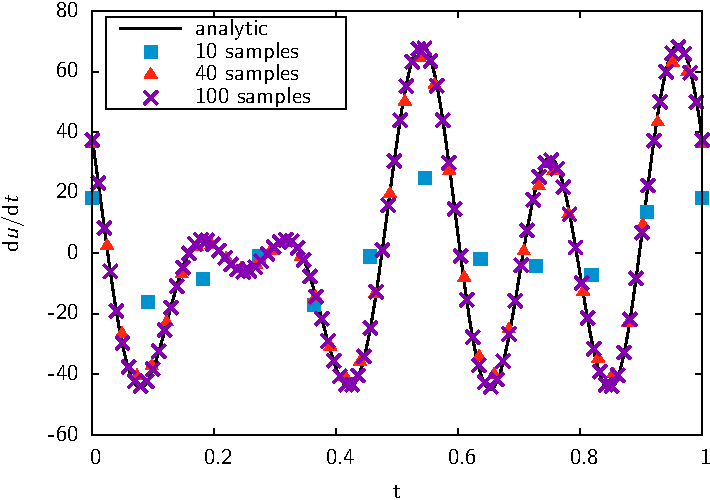
\includegraphics[width=.4\textwidth]{HB_OPERATOR_PPT_FD2.pdf}}
  \subfigure[FD 4\textsuperscript{th} order]{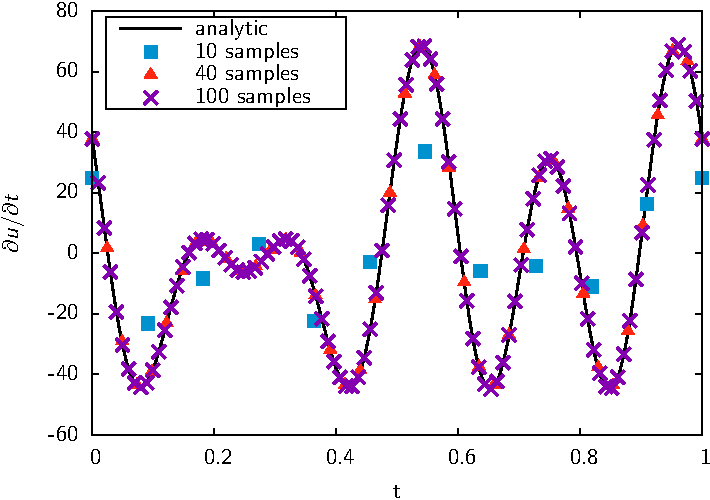
\includegraphics[width=.4\textwidth]{HB_OPERATOR_PPT_FD4.pdf}}
  \caption{Time-derivative estimation by the harmonic balance operator,
  the 2\textsuperscript{nd} order and 4\textsuperscript{th} finite-difference schemes.}
  \label{fig:hb_operator_sample}
\end{figure}
Four sampling levels
are tested for the HB operator: 7, 9, 11 and 13~time instances per period
corresponding to $N=3$, 4, 5 and 6, respectively.
For the FD schemes, the periodicity time interval is sampled by
10, 40 and 100 points.
For 40~samples, the 4\textsuperscript{th} order FD
scheme almost fits the analytical solution. On the other-hand,
the HB operator prediction is superimposed with the analytical solution
by using 11~samples, \emph{i.e.} $N=5$. Beyond that, further increasing the
number of harmonics (or samples)
does not improve the solution.

To quantitatively analyze the results, the 
$\mathcal{L}_2$-norm of the absolute error with respect to the analytical
derivative is computed for the different schemes and 
sampling levels (see Figure~\ref{fig:hb_operator_error}).
\begin{figure}[htp]
  \centering
   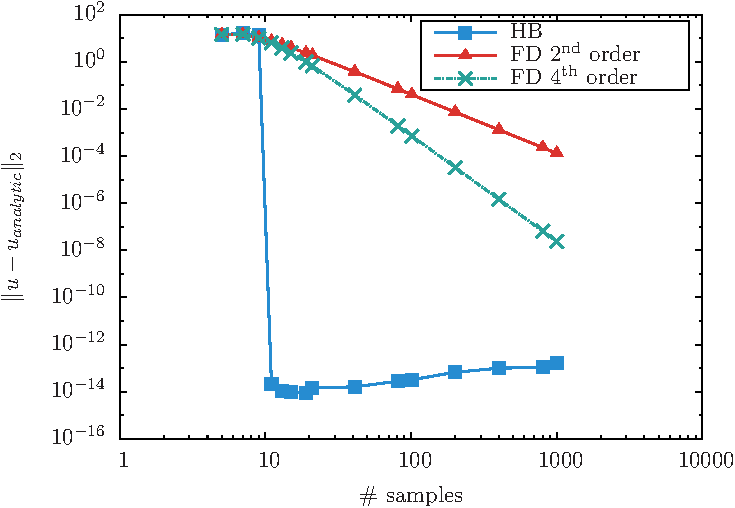
\includegraphics[width=.5\textwidth]{HB_OPERATOR_ERROR.pdf}
   \caption{$\mathcal{L}_2$-norm of the error for each time-derivative
   schemes.}
  \label{fig:hb_operator_error}
\end{figure}
As expected, the error of the 4\textsuperscript{th}~order FD
decreases faster  than the 2\textsuperscript{nd}~order for a given sampling level.
When the number of harmonics is low 
(\emph{i.e.} $N < 5$), the error is high for the HB operator. 
But as soon as $N \geq 5$, the error
drastically decreases to machine precision.
This illustrates the spectral accuracy as explained in 
Sec.~\ref{sub:spectral_accuracy}. In fact, the function defined
in Eq.~\eqref{eq:sum_sin_deriv} approximated by the spectral operator
is infinitely differentiable and periodic in $[0, T]$.
Thus, using the properties established in Sec.~\ref{sub:spectral_accuracy},
the convergence rate of the spectral operator is $\mathcal{O} (k^{-\infty})$
for $k > k_0$, here $k_0=5$. In this case, $k_0$
reflects the frequency content of the signal (namely $5$ harmonics).

The study of the convergence applied to the resolution
of turbomachinery harmonic balance computations will
be detailed in Chap.~\ref{cha:limitations_convergence}.
